\chapter{Patterns of premature fruit drop in tropical forest plants}

% \setcounter{page}{1} 
% \pagestyle{myheadings}
% \markboth{}{}\markright{} \rhead{\thepage} \setcounter{page}{1}
% \pagestyle{myheadings} \pagenumbering{arabic} \rhead{\thepage}
\section{Introduction}
Seed production is a critical element in the life cycle of a plant, giving rise to the next generation and thereby mediating population- and community- level dynamics (\cite{clarkArePlantPopulations2007a, maronHerbivoryEffectsPlant2006, turnbullArePlantPopulations2000, greenNonrandomDiversifyingProcesses2014}). Mortality events that happen in early life (from seed to seedling) can be a bottleneck for the recruitment of individuals to a population, with sometimes disproportionate effects on community composition (\cite{roughgardenRecruitmentDynamicsComplex1988}). This is particularly evident in plant communities, where seed availability can be the limiting factor determining plant population abundance and distribution (\cite{jamesDemographicProcessesLimiting2011,fennerEcologySeeds2005,rotherDemographicBottlenecksTropical2013}). A number of processes contribute to the success or failure of a developing seed, including nutrient availability, microclimatic conditions and the interactions between the plant and other organisms. For plant species relying on biotic pollination, visits from pollinators are crucial for reproductive success, often manifesting as a direct positive correlation between pollinator visitation rate and seed set (\cite{karronMultiplePollinatorVisits2006, steffan-dewenterPollinationSeedSet2001}). Following successful pollination, the developing seed might be a target for a range of enemies, including pre-dispersal insect seed predators, with deleterious effects on fitness. \par

While the importance of natural enemies of seeds and seedlings in the ecology of tropical forests has received much attention since Janzen’s (1970) and Connell’s (1971) seminal papers on the role of natural enemies in tropical forests (e.g. \cite{harmsPervasiveDensitydependentRecruitment2000, bagchiPathogensInsectHerbivores2014}), the bulk of research has focused on natural enemies attacking seeds or young seedlings after their dispersal from the mother plant (\cite{comitaTestingPredictionsJanzenConnell2014, hollEffectsSpeciesHabitat1997, leviTropicalForestsCan2019}). Although pre-dispersal seed mortality has been highlighted as a potentially important source of mortality and facilitator of high local plant diversity in tropical forests (\cite{ janzenHerbivoresNumberTree1970}), the fate of the plant’s progeny in the period prior to seed dispersal – as the fruit is developing – is relatively understudied in tropical forests (but see \cite{jonesDensitydependentPredispersalSeed2010}).

A commonly observed phenomenon in plants – including rainforest trees (S. Gripenberg, pers. obs.) – is that some fruits are prematurely abscised, i.e. drop from the mother plant prior to having completed their development. The ecological and agricultural research literature reports a number of causes of premature fruit drop (Table \ref{tab:causes}). For example, biotic and abiotic factors can contribute to changes in resource availability, triggering an individual to drop fruit which is unlikely to reach maturity and thereby minimising cost to the parent plant (\cite{stephensonFlowerFruitAbortion1981}). Damage by natural enemies can also lead to premature abscission, often through seed/fruit predation or pathogenic attack. Regardless of the exact mechanism causing premature fruit abscission, the resulting seed mortality could – if it reduces the number of viable seeds produced by the plant – have important effects on plant population and community dynamics. To our knowledge, this is the first study investigating patterns of premature fruit abscission in a tropical plant community and could provide insights into the coexistence of high numbers of tree species in tropical forests.

In this study we investigated patterns of premature fruit fall in the woody plant community (trees, shrubs, lianas) of Barro Colorado Island, Panama. Taking advantage of a long-term multi-species data set on seed and fruit rain, we quantified levels of premature fruit abscission for 268 plant species. Our overall aim was to explore the community-level patterns of premature fruit abscission. More specifically:

\begin{enumerate}
\item To describe and quantify interspecific variation in fruit abscission rates
\item To test whether variation in fruit abscission rates can be explained by plant phylogeny and selected plant traits (Table \ref{tab:traits})
\item To test whether premature fruit abscission rates are highest in plant species known to be attacked by internally-feeding, pre-dispersal insect seed predators
\end{enumerate} 

We hypothesised that:
\begin{itemize}
\item Seed enemies are the cause of some premature fruit drop
\item Plant species with traits hypothesised to make them more prone to enemy attack (Table \ref{tab:traits}) will have the highest rates of premature fruit abscission
\item Some traits are conserved among closely related plant species (Table \ref{tab:traits}), hence phylogeny may explain some of the variation between species 
\end{itemize}

\begin{sidewaystable}
\caption{Causes of premature fruit drop documented in the literature. For each cause, selected examples of studies are provided.}
\small
\begin{tabular}{|p{4cm}p{4cm}p{12cm}|}
\hline
        \textbf{Cause} &  & \textbf{e.g.} \\ \hline
        Resource limitation & Herbivory / Defoliation & \cite{cunninghamFruitSettingWatermelons1940,mehouachiDefoliationIncreasesFruit1995,yangBurstReactiveOxygen2015,jamesonResponsesIndividualPlants1963,janzenSeedingPatternsTropical1978,mcalisterResponseSoybeansLeaf1958,simmondsFurtherEffectsDefoliation1951,willsonAdaptiveDesignFloral1974} \\ \hline
         & Leaf shading & \cite{dashSevereShadingReduces2012,einhornABAShadingInduce2018,zhuAbscisicAcidEthylene2009,byersInfluenceLowLight1991,mayEffectShadingFruitfulness1963} \\ \hline
         & Nutrient depletion & \cite{bradburyComparativeStudyDeveloping1929,nightingaleEffectsNutrientConcentration1936,zhaoCottonGrowthPhysiological2003,bertaminiGrapevineGrowthPhysiological2005,martinez-alcantaraNitrogenuseEfficiencyYoung2012} \\ \hline
         & Frost & \cite{rodrigoSpringFrostsDeciduous2000,rodrigoSpringFrostDamage2006,addicottPhysiologyAbscission1955,addicottPhysiologicalEcologyAbscission1973,krugmanFreezingSpringTemperatures1966,tagliasacchiCytohistologicalCytochemicalFeatures2006,dorseyStudySterilityPlum1919} \\ \hline
         & Heat & \cite{zhouPhysiologicalResponseHeat2017,najeebEndogenousEthyleneConcentration2017} \\ \hline
         & Drought & \cite{reichardtPeptideSignalingDroughtinduced2020, udovenkoEffectDroughtOverheating1986,perez-perezResponseSweetOrange2008} \\ \hline
         & Leaf shading & \cite{dashSevereShadingReduces2012,einhornABAShadingInduce2018,zhuAbscisicAcidEthylene2009,byersInfluenceLowLight1991,mayEffectShadingFruitfulness1963} \\ \hline
        Damage to developing fruit & Seed predation & \cite{boucherEarlyDropNuts1979,dohanianControlFilbertWorm1944,lloydSexualStrategiesPlants1980,mattsonRoleInsectsDynamics1978,janzenSeedPredationAnimals1971,janzenSeedeatersVsSeed1969,janzenEscapeCassiaGrandis1971} \\ \hline
         & Fruit predation & \cite{planesWithintreeTemporalDistribution2014,bendaFruitAbscissionPhysalis2009,petzoldEffectHeliothisSubflexa2009, millerObservationsMelamphausFaber1932,phillipsImmatureNutfallCoconuts1940} \\ \hline
         & Pathogen attack & \cite{phillipsImmatureNutfallCoconuts1940,carterInjuriesPlantsCaused1939,akinsanmiFruitAbscissionMacadamia2016,teviotdaleAbscissionKernelQuality1997} \\ \hline
         & Genetic or developmental abnormalities & \cite{bradburyComparativeStudyDeveloping1929,krausSelfsterilityProblem1915,forinoEmbryosacsFrequencyOvules1987} \\ \hline
\end{tabular}
\label{tab:causes}
\end{sidewaystable}



\begin{sidewaystable}
\small
\begin{tabular}{|p{4cm}p{4cm}p{13cm}|}
\hline
        \textbf{Variable} & \textbf{Prediction} & \textbf{Hypothesis} \\ \hline
        Seed mass & Increased abscission with increased seed mass & Larger seeds are more valuable as a food source to potential seed predators (\cite{moegenburgSabalPalmettoSeed1996, fennerRelationshipCapitulumSize2002}). Additionally, large seeds might be exposed to predation from a wider range of seed predators (\cite{greigPredispersalSeedPredation1993, mucunguziBruchidsSurvivalAcacia1995}) and for a longer period of time (\cite{molesLatitudeSeedPredation2003}, but see \cite {molesSmallseededSpeciesHave2003}) \\ \hline
        Abundance of plant conspecifics & Increased abscission with increased abundance & Species with many conspecifics in the surrounding area are more prone to seed predator attack since the abundance of resources available to host-specific seed predators will be higher (\cite{janzenHostPlantsIslands1968}). \\ \hline
        Overlap in fruit production by other species & Increased abscission with decreased overlap & Species fruiting at times of the year when many other species fruit, experience lower percentage seed predation due to predator satiation. Species which fruit in tandem with others, called masting, use this to their advantage (\cite{kellyMastSeedingPerennial2002, kellyEvolutionaryEcologyMast1994, janzenSeedPredationAnimals1971}) \\ \hline
        Interannual variation in seed crop sizes & Increased abscission with decreased variation & Species with temporally predictable fruiting patterns are more prone to seed predator attack since they provide a more stable resource for seed predators (\cite{janzenSeedPredationAnimals1971,janzenWhyBamboosWait1976}) \\ \hline
        Endocarp investment (degree of investment in mechanical seed defences) & Increased abscission with decreased investment & Species that invest large amounts of resources in seed protection are less vulnerable to predation (\cite{benkmanImpactTreeSquirrels1995, rodgersonMechanicalDefenseSeeds1998,gathuaEffectsPrimatesSquirrels2000,kuprewiczMammalInsectPredation2010}) \\ \hline
        Average tree height & Increased abscission with increased height & Taller species are more apparent to enemies (\cite{gripenbergHighlyResolvedFood2019, janzenHostPlantsIslands1968}) \\ \hline

\end{tabular}
\caption{Plant traits hypothesised to influence susceptibility to attack by pre-dispersal enemies. If pre-dispersal enemy attack contributes to premature fruit abscission, we would also expect a link between these traits and premature fruit abscission rates.}
\label{tab:traits}
\end{sidewaystable}

%%%%%%%%%%%%%%%%%%%%%%%%%%%%%%%%%%%%%%%%%%%%%%%% METHODS %%%%%%%%%%%%%%%%%%%%%%%%%%%%%%%%%%%%%%%%%%%%%%%%

\section{Methods}
\emph{Study site}\\*
Barro Colorado Island (BCI; 9\degree9’N, 79\degree51’W), is a 16 km2 island situated in the Panama Canal, which supports semideciduous tropical forest with a 35m tall canopy. BCI became a reserve in 1923 and ecological studies have been carried out here for more than 100 years. The island is known for its 50 ha permanent forest dynamics plot – the first to be established within the CTFS-ForestGEO plot network in 1982 (\cite{anderson-teixeiraCTFSForestGEOWorldwideNetwork2015}). Within the 50-ha plot, all free-standing woody plants larger than 1 cm in diameter at breast height are mapped and measured at five-year intervals. The censuses have recorded 299 different tree species in the plot (\cite{ anderson-teixeiraCTFSForestGEOWorldwideNetwork2015}). Long-term studies of the forest dynamics plot at BCI have yielded considerable data on the spatial and temporal dynamics of tropical forests and led to many new insights into tropical forest ecology, including to species coexistence theory (e.g. \cite{conditBetaDiversityTropicalForest2002, comitaTestingPredictionsJanzenConnell2014, harmsPervasiveDensitydependentRecruitment2000}).

\emph{Seed Rain}\\*
Since 1987, weekly censuses of seed rain have been conducted within the 50-ha Forest Dynamics Plot as part of a research project coordinated by Dr S. J. Wright (Smithsonian Tropical Research Institute) e.g. (\cite{ wrightAnnualSpatialVariation2005, wrightGapdependentRecruitmentRealized2003, harmsPervasiveDensitydependentRecruitment2000, wrightNinoSouthernOscillation1999}). 250 seed traps are set along 2.7 km of trails within the plot, at 13.5-m intervals on alternating sides of the trail at locations between 4 and 10 m from the trail so that distances between neighbouring traps average 18.9 ± 3.6 m (mean ± 1 SD). Each trap consists of a 0.8m tall PVC frame and 1mm mesh covering a 0.5m\textsuperscript{2} square of forest floor. In weekly censuses of the traps, seeds, fruits and flowers are identified to species and counted. Fruits are categorised as mature (endosperm of seeds is fully developed) or immature (endosperm is not is fully developed). In this study, only observations of fruits and seeds were used and species were limited to woody plant species (trees, lianas and shrubs).

Species-specific proportions of prematurely abscised seeds were calculated as abscised seeds as a proportion of total seeds weighted by year.

\[proportion\,abscised = \frac{abscised\,seeds}{viable\,seeds + abscised\,seeds}\ \]

Where;\\*
Abscised seeds = immature fruits × mean number of seeds per fruit\\*
Viable seeds = single diaspores + (mature fruits × mean number of seeds per fruit)

Data on species-specific mean numbers of seeds per fruit were obtained from S. J. Wright.
For each species, we first calculated yearly premature fruit abscission rates by pooling the data from all individual seed traps in which the species occurred for each full calendar year in the data set (1988 to 2018; n = 31 years). Since the majority of species fruit only once during a calendar year, and since few species fruit in the December/January period, this approach will typically generate data on overall fruit abscission rates for individual fruiting events. We used the species-specific averages of these values for the phylogenetic analyses.

Of the 311 woody plant species in the full seed rain dataset, 268 had data available regarding the typical number of seeds per fruit (required to calculate the numbers of abscised and viable seeds). To ensure a reasonable sample size of fruits, species were excluded from the analysis if total seeds (abscised + viable) across all years was lower than 50, leaving 201 species in the dataset (Table \ref{tab:summary}).

\begin{table}
    \centering
    \caption{Summary of seed rain dataset}
    \small
    \begin{tabular}{lrrrrr}
        \textbf{Lifeform} &     \textbf{Mature fruit} &      \textbf{Single diaspores} &     \textbf{Immature fruit} &      \textbf{Species} &         \textbf{Families} \\
        Liana &                83,785  &                39,052  &                74,917  &     55  &                         18  \\
        Midstory tree &                49,604  &                37,480  &              105,284  &      21  &                         16  \\
        Shrub &                   4,491  &                54,425  &                   8,084  &     20  &                         11  \\
        Canopy tree &              312,650  &              601,120  &              386,617  &               66  &                         29  \\
        Understory tree &              184,530  &              363,429  &              101,473  &      39  &                         19  \\ \hline
         Total &              635,060  &          1,095,506  &              676,375  &            201  &                         93  \\ \hline
    \end{tabular}
    \label{tab:summary}
\end{table}

\emph{Plant phylogeny and trait data}\\*
Data on traits listed in Table \ref{tab:traits} was obtained from a variety of sources as detailed in \cite{gripenbergHighlyResolvedFood2019} and \cite{wrightFunctionalTraitsGrowth2010}. Information on the presence and abundance of seed predators on individual plant species was obtained from a study by \cite{gripenbergHighlyResolvedFood2019} in which insects were reared from seeds or fruits collected on BCI. A phylogeny which included 197 of the plant species in our data set was provided by David Erickson (Smithsonian Institution).  The phylogeny was constructed following methods in \cite{kressPlantDNABarcodes2009}.

\emph{Analysis}\\*
Before conducting any further analyses I assessed co-variance of plant traits using Spearman’s rank correlation coefficients for all pairwise trait combinations.

To determine whether premature seed abscission rates were influenced by species-specific plant traits (Table \ref{tab:traits}), I constructed generalised linear mixed-effects models (GLMMs) with a Binomial probability structure using the 'glmer' function in the R package lme4 (\cite{batesLme4LinearMixedEffects2020}). For the response variable I used a two column data structure of prematurely abscised seeds and viable seeds, which was created using the 'cbind' function. The number of successes was equal to the estimated number of prematurely abscised seeds and the number of failures was equal to the number of fully developed seeds. This method enabled me to give higher weighting to species with a greater sample size of seeds (i.e. a higher number of total seeds). Since the data set included multiple observations per species (one value for each year of the study period in which fruits were observed in the seed traps), the models included species, year and their interaction as random effects, structured as: (1 \textbar Year)+(1 \textbar Species)+(1 \textbar Year:Species). Due to uneven sampling of trait values in the dataset, when using a maximal model structure to test for combined effects of plant traits on the proportion of abscised seeds and interactions between them, the sample size was severely reduced (from 201 species to 89). For this reason, only uni-variate mixed effects models are presented here. Each of the selected plant traits were tested independently as fixed effects. Two of the variables (local abundance and seed dry mass) were log transformed to reduce skew in the data caused by extreme values. Diagnostic plots were generated using the package DHARMa (\cite{hartigDHARMaResidualDiagnostics2020}) to assess goodness of fit. The final models were then visualised in ggplot (\cite{wickhamGgplot2CreateElegant2020}) by overlaying the predicted values, generated using the package effects (\cite{foxEffectsEffectDisplays2019}), onto a scatter plot of the data.

Since phylogenetic non-independence of species could potentially result in spurious patterns between seed abscission rates and plant traits, I ran a parallel set of phylogenetic generalised least squares (PGLS) models in which the relationship between premature seed abscission rates and individual plant traits were analysed while accounting for phylogenetic non-independence of closely related species. PGLS were run using the function 'pgls' in the R package caper (\cite{ormeCaperComparativeAnalyses2018}). Since the 'pgls' function does not allow random effects, data for individual species had to be pooled across the full 30-year study period to obtain one species-specific estimate of fruit abscission (=the mean species-specific fruit abscission rate, expressed as a proportion). The results from these models were qualitatively similar to the results from the GLMM and will not be presented here.

To explore if shared ancestry contributes to similarities in premature seed abscission among species within the community, I estimated the phylogenetic signal (the tendency for related species to be more similar than species drawn at random from the phylogenetic tree) in the proportion of seeds prematurely abscised. Both Pagel’s lambda (\cite{pagelInferringHistoricalPatterns1999, pagelInferringEvolutionaryProcesses1997}) and Blomberg’s K (\cite{blombergTestingPhylogeneticSignal2003}) were estimated, using 'phylosig' in the R package phytools and 'phylosignal' in picante respectively (\cite{revellPhytoolsPhylogeneticTools2020, kembelPicanteIntegratingPhylogenies2020}). The values of these indices vary from 0 (where phylogenetic and trait similarity are totally independent) to 1 (where the traits are completely explained by shared ancestry under Brownian motion). The 'contMap' function in the R package phytools (\cite{revellPhytoolsPhylogeneticTools2020}) was used to visualise phylogenetic signal in premature seed abscission as a continuous trait mapped onto the phylogenetic tree.


%%%%%%%%%%%%%%%%%%%%%%%%%%%%%%%%%%%%%%%%%%%%%%%% RESULTS %%%%%%%%%%%%%%%%%%%%%%%%%%%%%%%%%%%%%%%%%%%%%%%%

\section{Results}
My results indicate that premature fruit abscission in the forest dynamics plot is common. Of the 1,311,706 fruits collected in the seed rain traps across all years and plant species, 676,533 were immature (52\%). Taking into account single diaspores collected in the traps and the mean number of seeds per fruit for each species, of 8,996,317 total seeds sampled, 3,270,289 were abscised prematurely (36\%). No prematurely abscised fruits were collected for 30 species (Figure \ref{fig:hist}), the remaining 171 species all abscised some seeds with 49 abscising more than 50\% of total seeds on average across the 31-year study period.

\begin{figure}[!h]
\centering
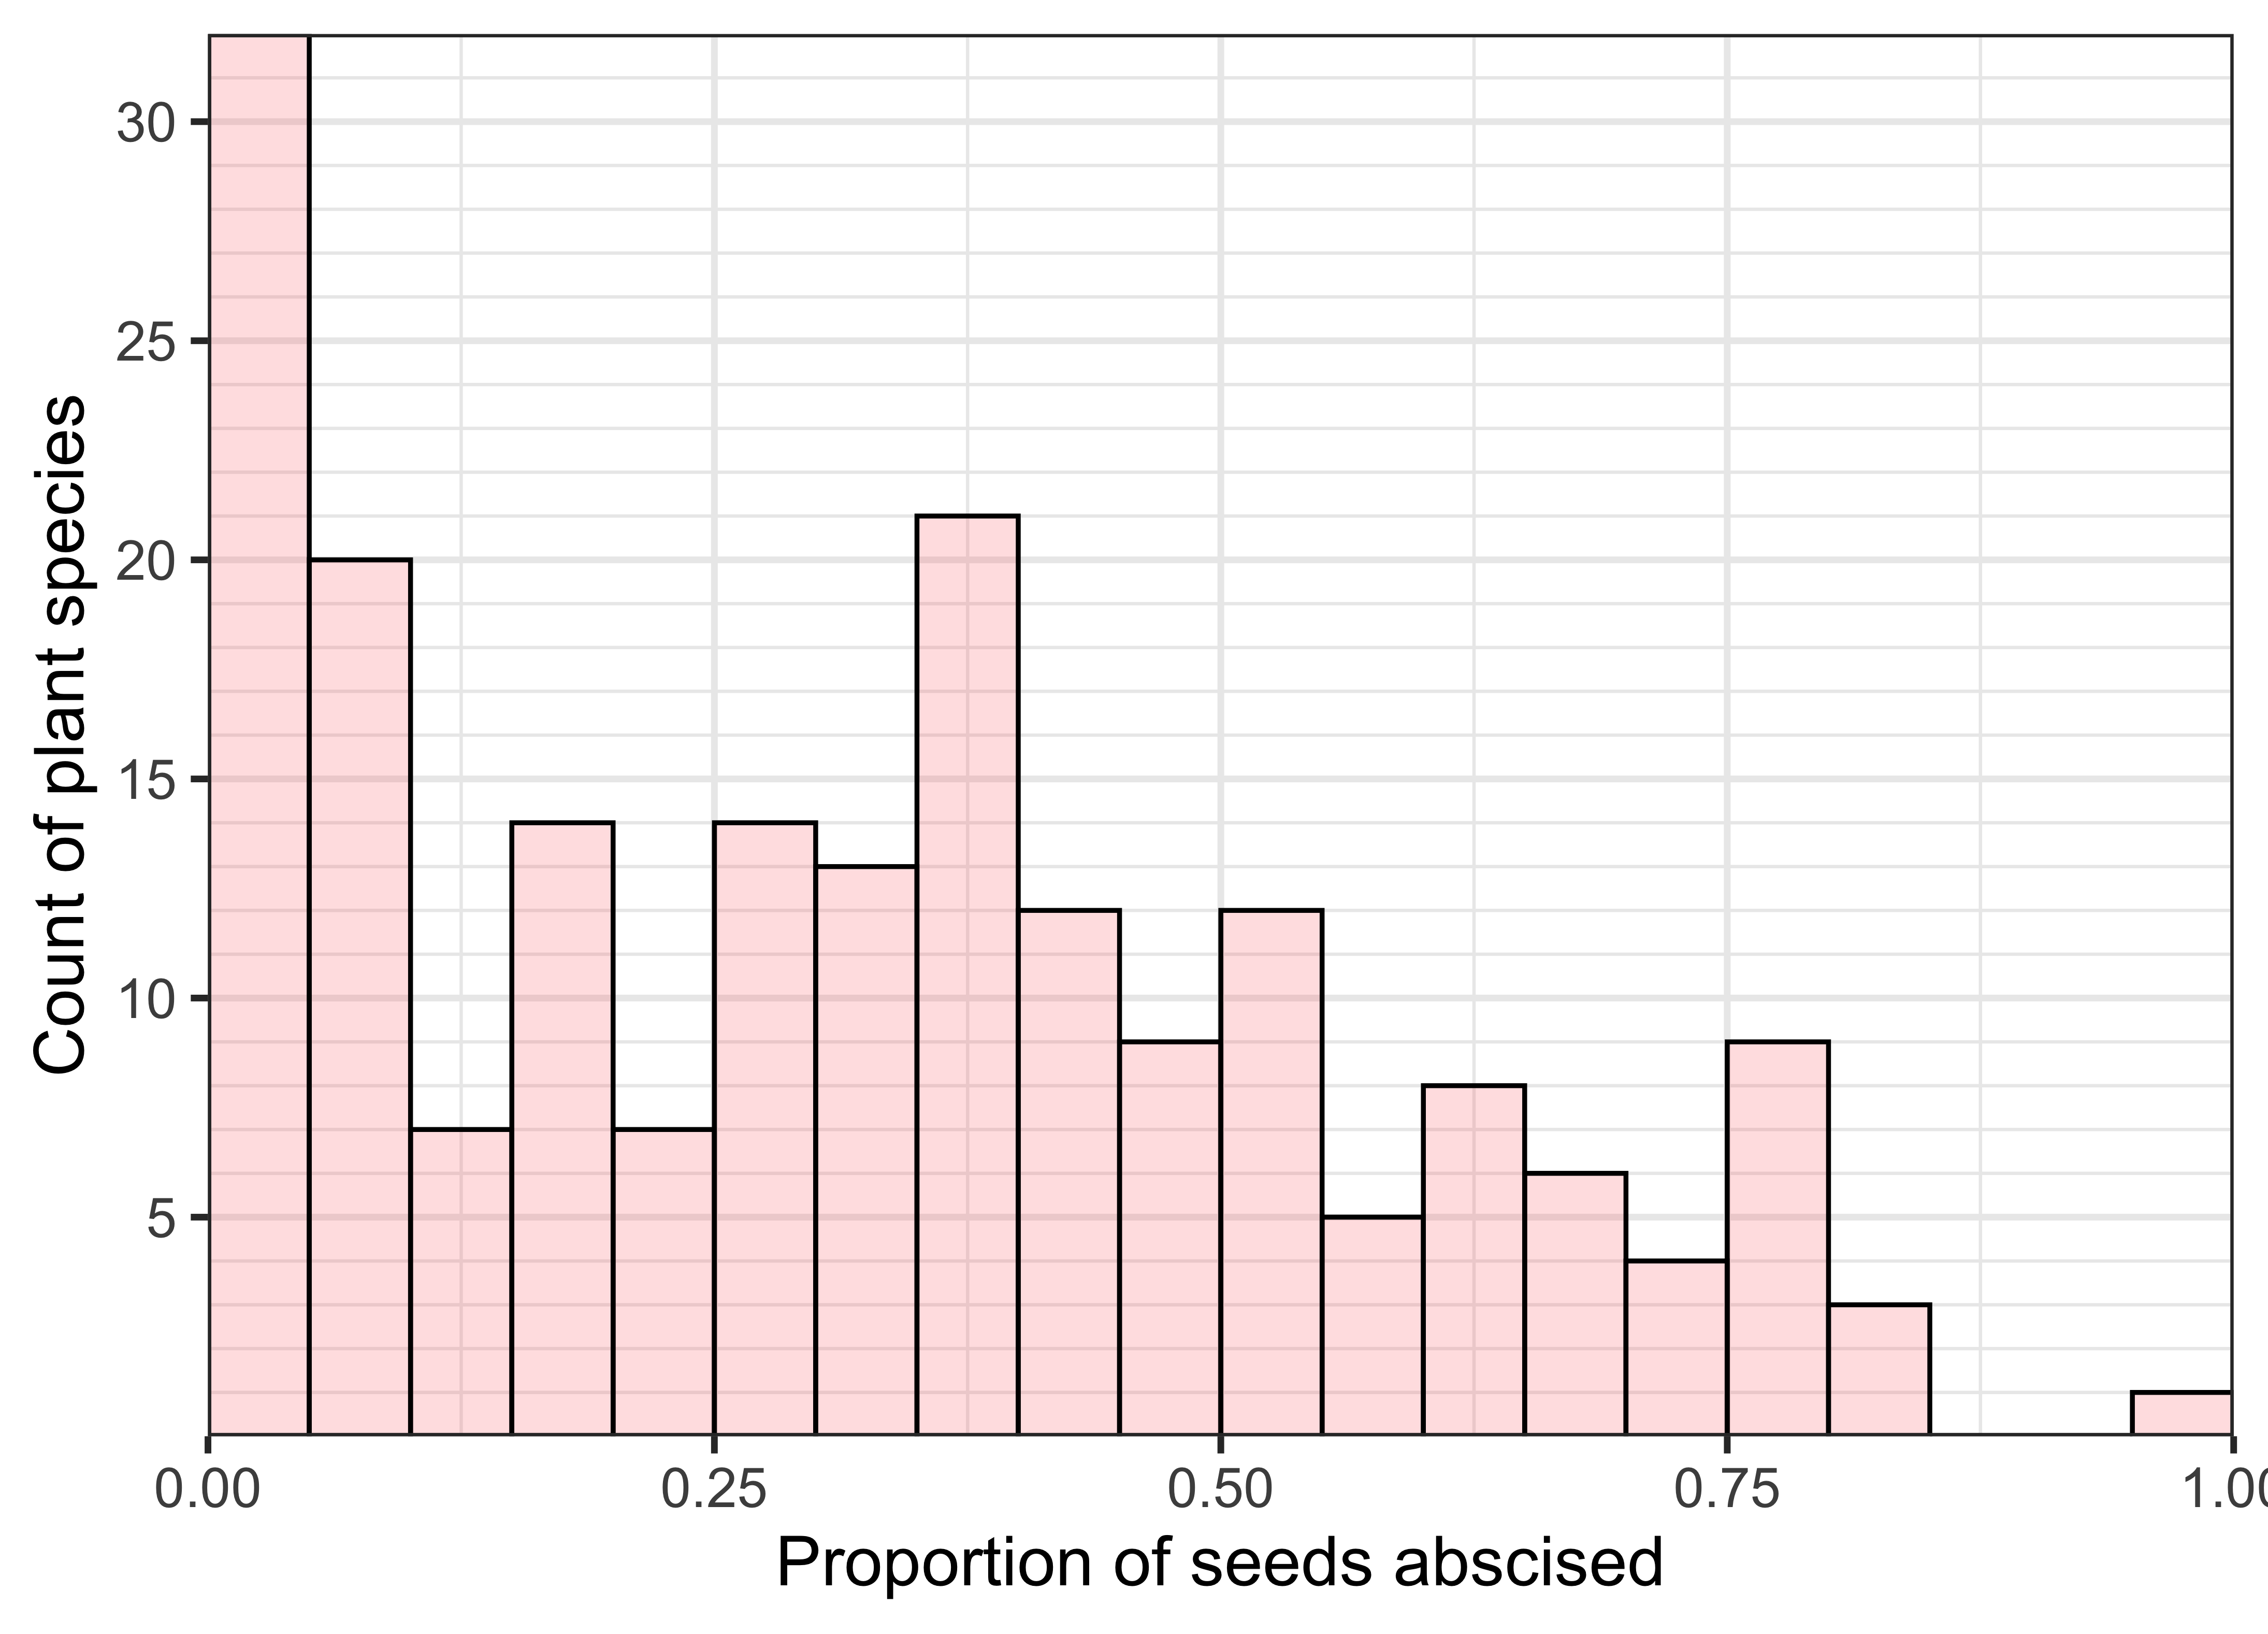
\includegraphics[width=10cm]{overallHist.png}
\caption{Histogram showing the frequency distribution of the proportion of prematurely abscised seeds across species in the woody plant community of BCI}
\label{fig:hist}
\end{figure}

\begin{figure}[!h]
\centering
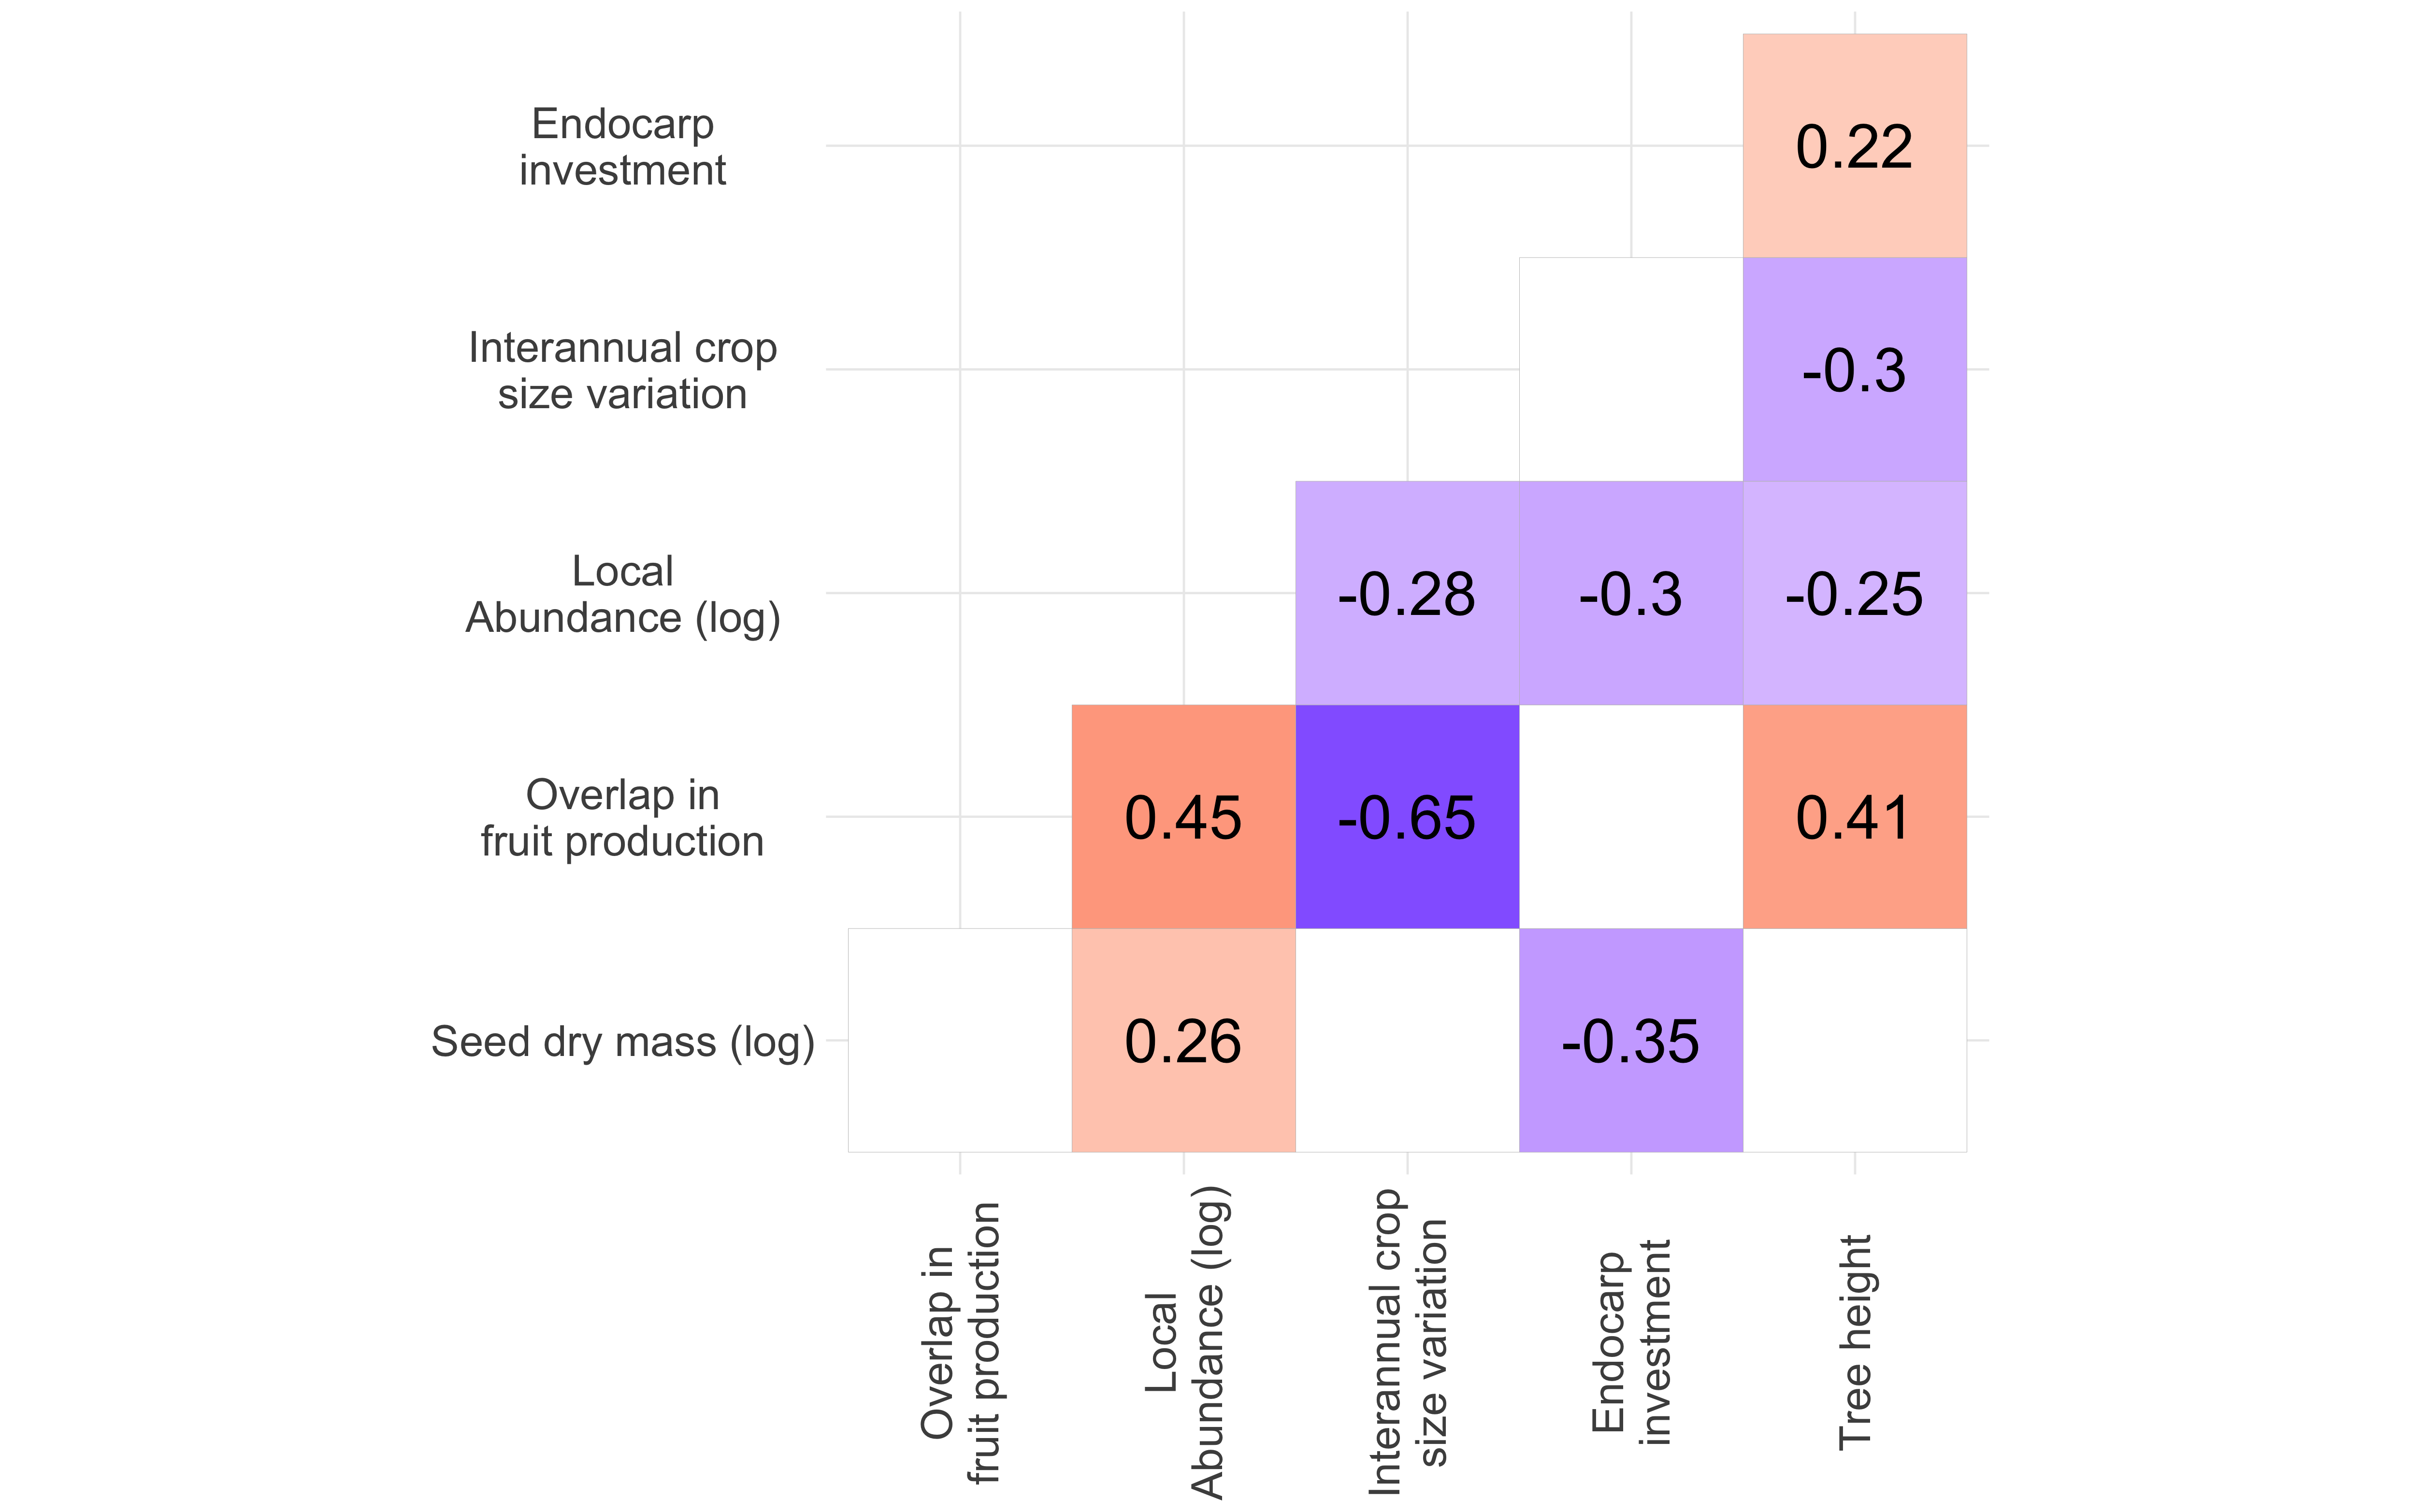
\includegraphics[width=10cm]{traitsCorr.png}
\caption{Correlations between plant traits. Numbers and colours show Spearman’s rank correlation coefficient (red = positive, blue = negative), blank tiles indicate correlations for which p = \textgreater0.05}
\label{fig:corrmat}
\end{figure}

Plant traits did not correlate strongly (Figure \ref{fig:corrmat}). Spearman's rank correlation coefficients were all below 0.70, the level below which multicollinearity is not deemed to be a problem (\cite{tabachnickUsingMultivariateStatistics1989}).
All of the selected plant traits, excluding endocarp investment, demonstrated a statistically significant relationship with the proportion of seeds abscised (Figure \ref{fig:glmms}, Table \ref{tab:glmms}). Locally abundant species had higher premature fruit abscission rates than rarer species. Taller tree species prematurely abscised a higher proportion of seeds, as did species with greater seed mass. Species fruiting at times of the year when few other species fruit had lower levels of premature seed abscission. Species not known to be attacked by insect seed predators had lower levels of premature seed abscission than species from which seed predators have been reared (Figure \ref{fig:seedbox}, Table \ref{tab:glmms}).

\begin{table}[!h]
    \centering
    \caption{Results of uni-variate generalised linear mixed models for plant traits as predictors of proportion of seeds abscised.}
        \begin{tabular}{lrrrr}
        \textbf{Plant trait} & \multicolumn{1}{c}{\textbf{Estimate}} & \multicolumn{1}{c}{\textbf{SE}} & \multicolumn{1}{c}{\textbf{z-value}} & \multicolumn{1}{c}{\textbf{p}} \\
        log (Local abundance) & 1.280 & 0.320 & 4.0 & \textless 0.001 \\
        log (Overlap in fruit production) & 0.010 & 0.002 & 4.8 & \textless 0.001 \\
        Interannual crop size variation & -0.652 & 0.294 & -2.2 & 0.026 \\
        Endocarp investment & -0.701 & 0.725 & -1.0 & 0.334 \\
        Average tree height & 0.064 & 0.019 & 3.4 & \textless 0.001 \\
        log (Seed dry mass) & 0.915 & 0.179 & 5.1 & \textless 0.001 \\
        Presence of seed predator & 1.435 & 0.390 & 3.7 & \textless 0.001
        \end{tabular}
\label{tab:glmms}
\end{table}

\begin{figure}[!h]
\centering
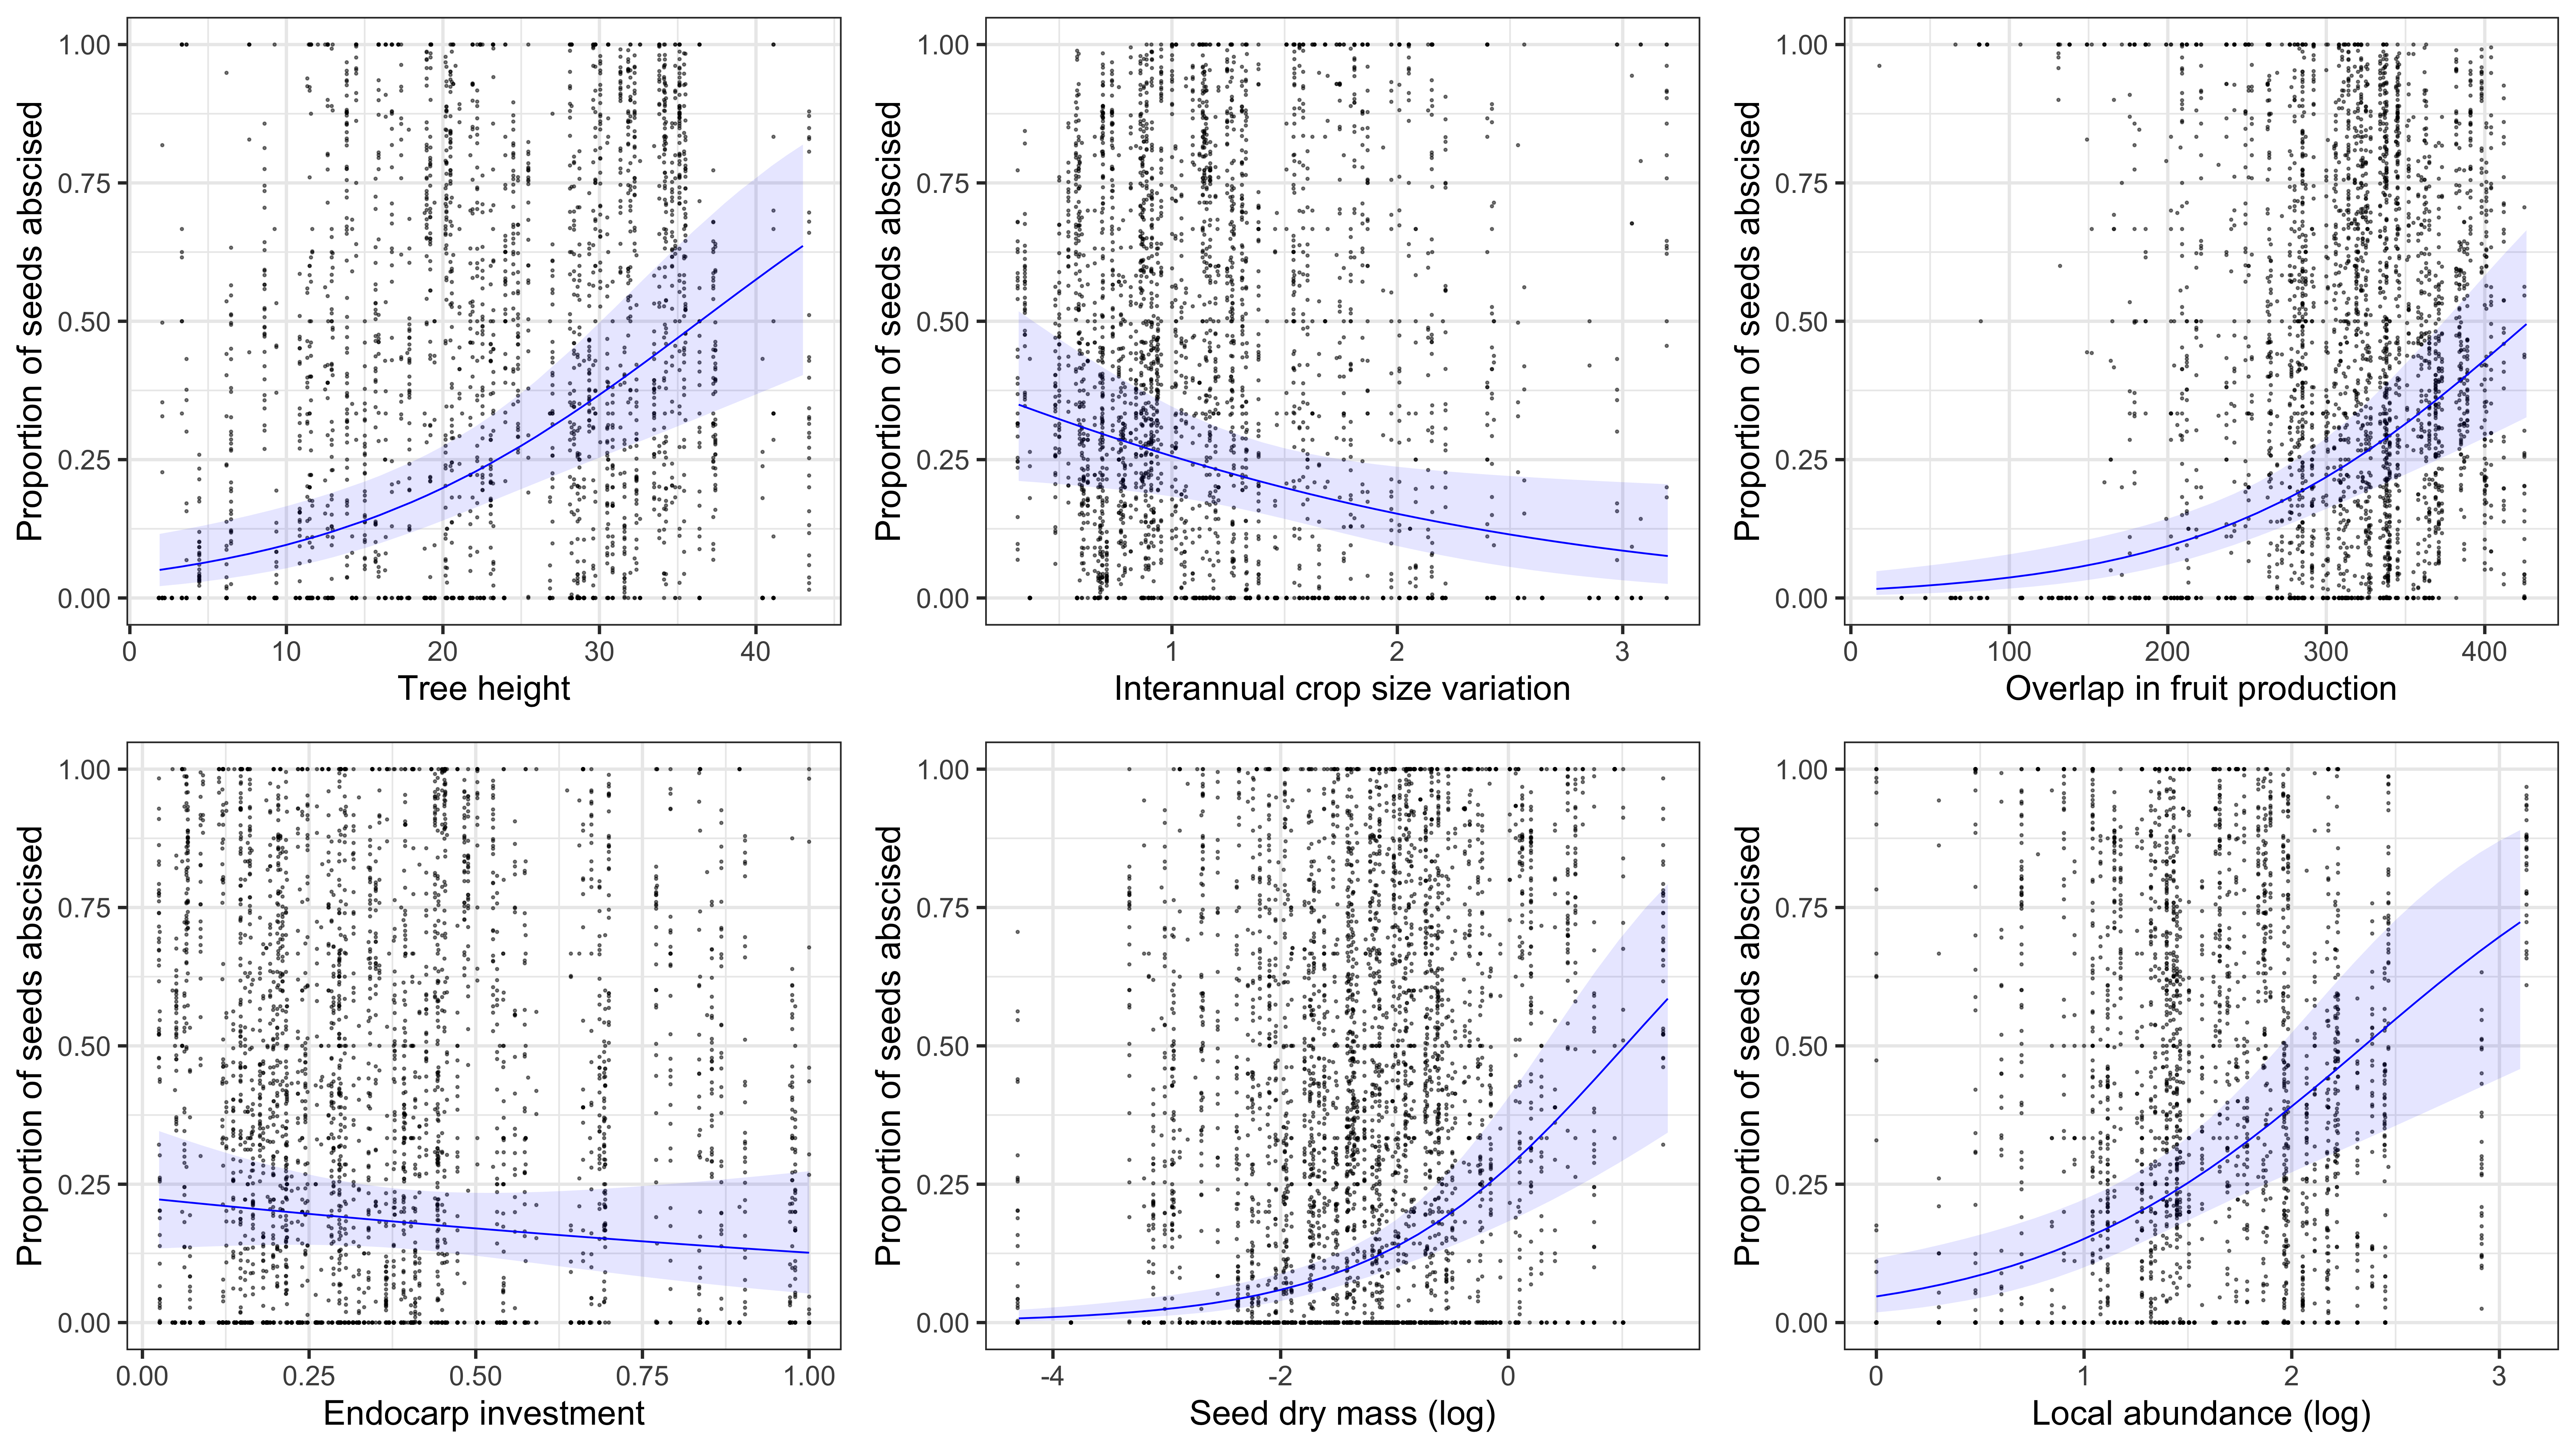
\includegraphics[width=15cm]{glmms.png}
\caption{Relationships between premature seed abscission rates and plant traits hypothesised to reflect likelihood of attack by seed enemies. Lines are GLMM model fits with 95\% confidence intervals.}
\label{fig:glmms}
\end{figure}

\begin{figure}[!h]
\centering
\includegraphics[width=15cm]{predPres.png}
\caption{Premature fruit abscission and presence of insect seed predators based on observations by \cite{gripenbergHighlyResolvedFood2019}. Panel (a) includes all insect seed predators, panel (b) shows the presence of insect orders Coleoptera, Hymenoptera and Lepidoptera independently. Species not known to be attacked by insect seed predators had lower levels of seed abscission than species from which seed predators have been reared (GLMM; Table \ref{tab:glmms}).}
\label{fig:seedbox}
\end{figure}

\begin{figure}[!h]
\centering
\includegraphics[width=15cm]{ContMap.png}
\caption{Phylogenetic signal of premature fruit abscission for 197 species. Blue represents an average proportion of abscised seeds equal to 1 and red is equal to 0. Phylogenetic signal of premature fruit abscission was estimated using Pagel’s lambda (\textlambda = 0.30; p = \textless0.005) and Blomberg's K (K = 0.00, p = 0.12)}
\label{fig:phylotree}
\end{figure}

Mapping rate of premature seed abscission across the phylogenetic tree, it is notable that species which have an extremely low trait value (close to 0\% of seeds are abscised) are often close together in the phylogenetic tree. Most other species have intermediate trait values and species with high trait values seem to be randomly spread throughout the tree (Figure \ref{fig:phylotree}). Estimates of phylogenetic signal for proportion of seeds abscised were relatively low.
Blomberg’s K phylogenetic signal estimate for proportion of seeds prematurely abscised was very low (K = 0.00, p = 0.12), suggesting large trait differences among close relatives. Pagel’s lambda estimate, however, was notably higher (\textlambda = 0.30, p = \textless 0.005). The exact definition of “high” and “low” values of lambda and K varies among studies (\cite{kamilarPhylogeneticSignalPrimate2013}), making it difficult to assess the level of phylogenetic non-independence in rates of premature fruit abscission.

%%%%%%%%%%%%%%%%%%%%%%%%%%%%%%%%%%%%%%%%%%%%%%%% DISCUSSION %%%%%%%%%%%%%%%%%%%%%%%%%%%%%%%%%%%%%%%%%%%%%%%%

\section{Discussion}
Seed production and survival mediates the composition of plant communities. While studies on the fate of seeds that have dispersed from the parent plant have found natural enemies to be important for the coexistence of plant species in tropical forests, we do not know if natural enemies such as pre-dispersal seed predators attacking seeds in the canopy play a similar role. I used a dataset of fruit drop for 201 woody plant species collected in a Panamanian forest (Barro Colorado Island) over a 31-year period to assess interspecific patterns of premature fruit abscission. We found that plant traits hypothesised to be associated with with a higher risk of enemy attack correlated with increased rates of premature fruit abscission and that premature abscission rates were higher in plants species which are known to be attacked by pre-dispersal insect seed predators. This suggests that seed enemies may be the cause of some premature fruit abscission with potential implications for plant diversity maintenance in tropical forests.

\emph{Plant traits as predictors of premature fruit abscission}\\*
Traits hypothesised to be more prone to seed predator attack were associated with higher rates of premature fruit abscission in woody plants. This is in agreement with previous studies of leaf herbivory in tropical forests, which have found that interspecific variation in enemy attack can be explained by variation in traits between species (\cite{cardenasPlantTraitsPredict2014, schuldtPlantTraitsAffecting2012}). Plant species which had traits associated with potential abundant resources for enemies, such as a large seed mass and high local abundance of con-specifics, prematurely abscised a larger proportion of their developing seeds. In addition to providing a larger food resource, species with larger seeds may also be be exposed to pre-dispersal seed predators for a longer period of time, as larger seeds take longer to develop (\cite{molesLatitudeSeedPredation2003}). A high local abundance of con-specific plants are more likely to be colonised by, and can support a larger population of, host-specific seed predators (\cite{pacalaHerbivoresPlantDiversity1992, hanskiSpatiallyRealisticTheory2001}). In this study, taller plant species had higher rates of premature fruit abscission. Canopy trees are likely to have larger seed crops and be more apparent to seed predators than understory trees and shrubs (\cite{janzenHostPlantsIslands1968, castagneyrolPlantApparencyOverlooked2013}). Both a greater average height and  high local abundance of con-specifics could increase the apparency of species to seed predators and my results are consistent with studies which found lower insect herbivore infestations on host trees which were concealed by non-host plants (\cite{floaterHabitatStructureEgg2000, hughesNeighboringPlantSpecies2012}). Herbivory is also known to cause premature fruit drop and traits which increase apparency to seed predators probably also increase apparency to herbivores, possibly inflating the effect on fruit abscision rate in these results.

 Increased overlap in fruit production with other plant species corresponded to an increase in the rate of premature fruit abscission. This supports the hypothesis that an abundance of fruit at the wider community-level supports a greater population of pre-dispersal enemies which leads to higher levels of attack and premature abscission. However, this would not be the case if seed predators or other enemies triggering premature fruit drop were purely host specific and could have the opposite effect of reducing apparency of host plants. It is possible that the effect of host-specific seed predators on premature fruit abscission is masked by the effect of other non-host-specific pre-dispersal enemies. Masting behaviour, whereby species fruiting in tandem with many other species benefit from predator satiation, is an example of when plant species will use the non-specificity of predators to their advantage (\cite{kellyEvolutionaryEcologyMast1994}). An additional benefit of masting is that the intermittent and unpredictable reproduction of host plants can cause local extinctions of seed predator populations (\cite{satakeSpatialDynamicsSpecialist2004,yasakaMastingBehaviorFagus2003}). We saw that plant species with greater variation in crop size between years had lower rates of premature fruit abscission, which could be due to a temporally unstable food resource reducing predator populations.

I expected a negative relationship between investment in mechanical seed defences and fruit abscission rates, as seeds with less protective tissue would be more vulnerable to attack, however there was no significant relationship between these traits. The effect may be diluted, as interspecific variation in seed defence would be irrelevant for host-specific seed predators. Additionally, mechanical defences may be less important for insect predators, as smaller seed predators can exert greater forces relative to their body mass. Previous work on Barro Colorado Island found that seed toughness per unit mass decreases with increasing seed mass and concluded that smaller seed predators should be less sensitive to the relatively greater toughness of small seeds (\cite{frickeMechanicalDefenceAdvantage2016}).

\emph{Phylogeny as a predictor of premature fruit abscission}\\*
While there was some evidence of phylogenetic clustering for low rates of fruit abscission there was no clear phylogenetic signal in premature fruit abscission. There are however, distinct differences in fruit abscission rates between species, suggesting that whilst some aspects of fruit abscission may be determined by genetics and conserved evolutionarily, the dynamics of biotic and abiotic factors in space and time play a larger role. This theory is consistent with a similar study, which found little evidence of phylogenetic signal in herbivore abundance and host plant traits (\cite{whitfeldPredictingTropicalInsect2012}).

\emph{Pre-dispersal seed predators as the cause of some premature fruit abscission}\\*
A key aim of this project was to assess whether pre-dispersal seed enemies are the cause of some premature fruit abscission in tropical plants. I found that plant species known to be attacked by insect pre-dispersal seed predators had higher levels of fruit abscission, suggesting that they may play a role, however the magnitude of their effect is unknown and is likely obscured by other mechanisms which are known to cause premature fruit abscission.

\section{Conclusions and next steps}
My mini-project on the community-level patterns of premature fruit abscission in the BCI plant community suggests that for many species, premature fruit abscission might be a major driver of seed mortality. Moreover, the patterns of fruit abscission suggest that enemies such as pre-dispersal insect seed predators might be contributing to premature fruit abscission. For part of my PhD, I will explore the phenomenon and its potential implications for species coexistence in the forest of BCI.

\emph{Temporal patterns of fruit abscission}\\*
Whilst analysing the dataset for this study, I noticed large variation in premature fruit abscission at an intraspecific level, with striking temporal trends (see \textit{Hieronyama alchorneoides} and \textit{Mascagnia divaricata}, Figure \ref{fig:temporal}). It is likely that factors such as weather and population sizes influence fruit abscission at the level of the individual across time. I plan to investigate this using a subset of the same data used in this mini-project.

\emph{Spatial patterns of fruit abscission}\\*
The Janzen-Connell hypothesis for species coexistence in tropical forests predicts that seed mortality due to natural enemies will be highest closest to adult plants of the same species and in areas of high conspecific density. If insect seed predators or other specialist pre-dispersal seed enemies contribute to immature fruit abscission, we might therefore expect fruit abscission rates to be highest in parts of the forest where the density of conspecific tree individuals is highest. I will be able to test this hypothesis using the seed rain dataset.

\begin{figure}[!h]
\centering
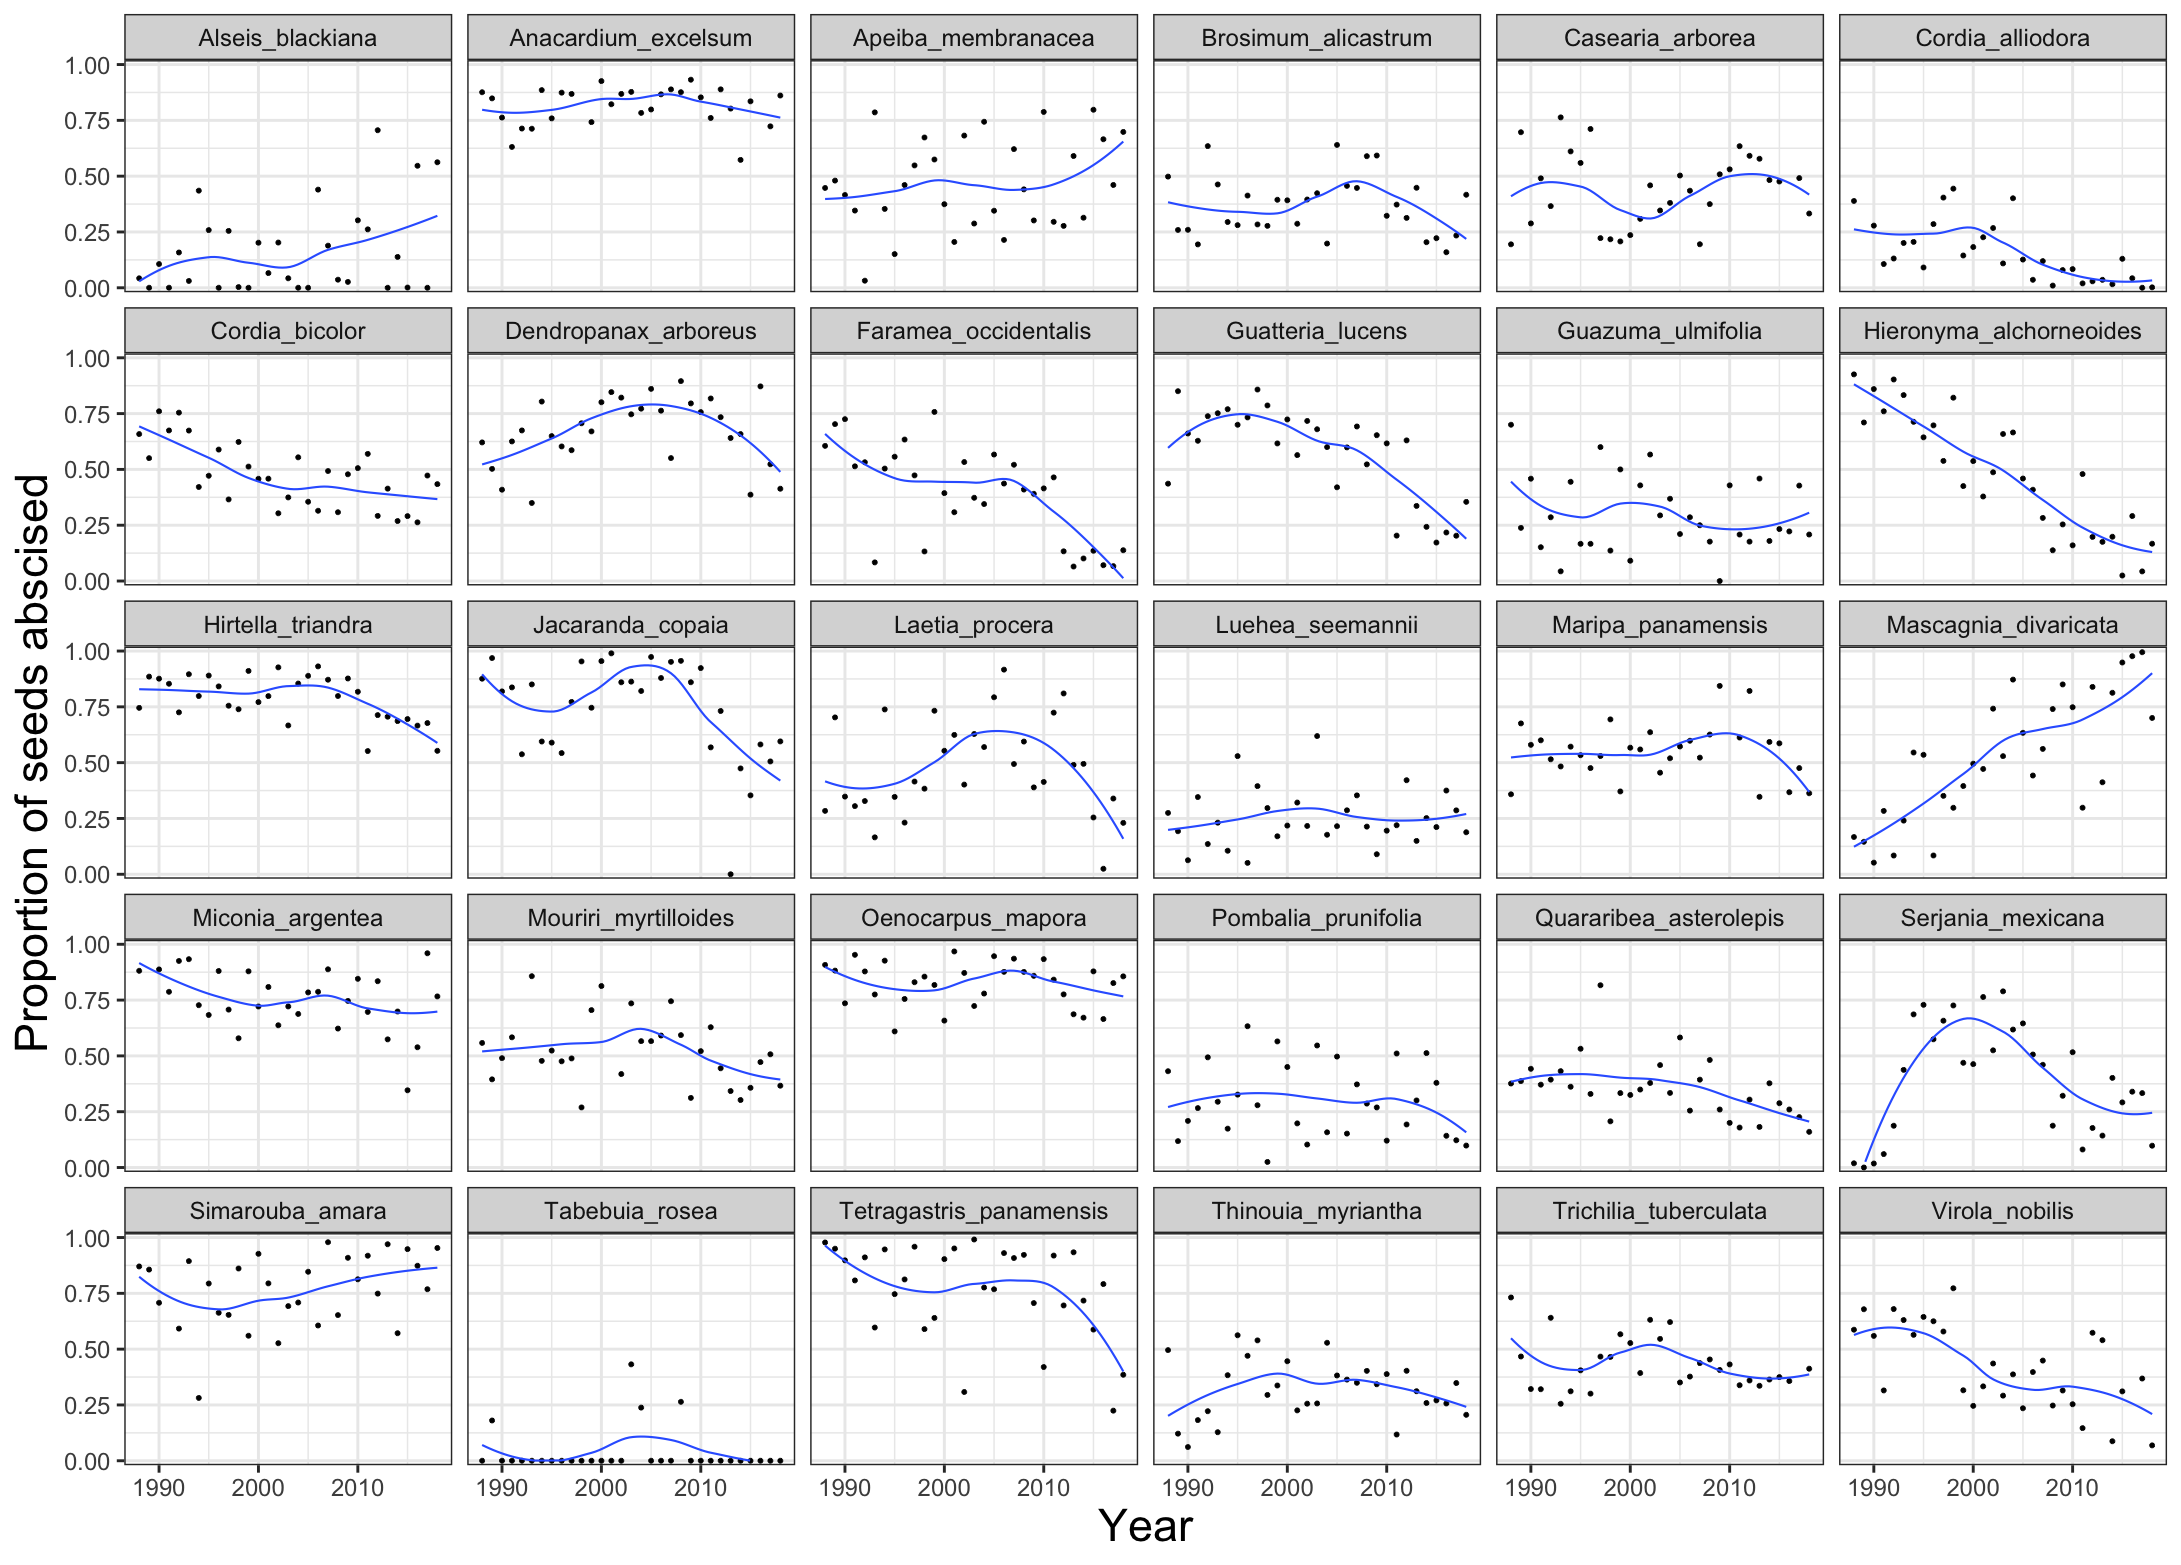
\includegraphics[width=15cm]{yearBySp.png}
\caption{Temporal trends in the rate of premature seed abscission for a subset of plant species. These are the absolute numbers of seeds abscised as a proportion of total seeds per year. A smoothed line of conditional means has been added to aid visualisation.}
\label{fig:temporal}
\end{figure}